\section{Multivariate Distribution and its Generalisations}
%%%%%%%%%%%%%%%%%%%%%%%%%%%%%%%%%%%%%%%%%%%%%
\subsection{Matrix algebra}

The main tool of the course is matrix algebra. We therefore repeat the most important convepts. The matrix $\mA$ is said to be \term{symmetric} if $\mA^\top=\mA$. It is \term{orthogonal} if $\mA\mA^\top=\mA^\top\mA=\mI$, i.e. if the columns are orthogonal. The elements of the pair ($\lambda, \boldsymbol{\gamma}$) are called \term{eigenvalue} and \term{eigenvector} respectivelly if they satisfy $\mA\boldsymbol{\gamma}=\lambda \boldsymbol{\gamma}$ and $\boldsymbol{\gamma}\ne \zero$. $\lambda$ can be found as the solution of $\det(\mA-\lambda \mI)$. Recall that the \term{trace}, $\tr{\mA}$, of a matrix is the sum of the diagonal. We also have the formulas:
$$
    \det{\mA} = \prod_{i=1}^p \lambda_i
    \quad
    \tr{\mA} = \sum_{i=1}^p \lambda_i.
$$
For a symmetric matrix we may find the \term{Jordan decomposition}. Let $\Lambda = \textrm{diag}\{\lambda_1, \dots, \lambda_p\}$ and $\Gamma = (\boldsymbol{\gamma_1}, \dots, \boldsymbol{\gamma_p})$. Then we have:
$$
    \mA=\mG\mL\mG^\top.
$$
For a symmetrix matrix $\mA$ and a vector $\x$ we define the \term{quadratic form}:
$$
    Q(\x) = \x^\top \mA \x = \sum_{i=1}^p\sum_{j=1}^p x_i A_{ij} x_j.
$$
\begin{theorem}
    Transforming $\y=\mG^\top\x$ we obtain 
    $$
        Q(\x) = \sum_{i=1}^p \lambda_i y_i^2.
    $$
\end{theorem}
A matrix is said to be \term{positive definite} if $Q(\x)>0$ for all $\x\ne0$ and positive semi definite if $Q(\x)\geq0$ for all $\x\ne0$. We write $A>0$ and $A\geq 0$ respectivelly. 
\begin{theorem}
    The symmetric matrix $A$ is positive definite iff $\lambda_i > 0$ for all $i$.
\end{theorem}
\begin{proof}
    Using the transform of the previous theorem we find 
    $$
        \lambda_1 y_1^2 + \dots + \lambda_p y_p^2 > 0 \quad\forall \y\in\R^p \Leftrightarrow \lambda_i > 0 \quad\forall i. 
    $$
\end{proof}
From this we obtain two more usefull results. 
\begin{enumerate}
    \item If $\mA>0$ the inverse exists and the determinant is $>0$
    \item If $\mA>0$ there exists a unique positive definite square root with decomposition:
    $$
        \mA^{1/2} = \mG\mL^{1/2}\mG^\top.
    $$
\end{enumerate}

%\subsection*{Lecture 1}
%%%%%%%%%%%%%%%%%%%%%%%%%%%%%%%%%%%%%%%%%%%%%%%%%%%%%%%%
\subsection{Random vectors and distributions}

A \term{random vector} $\X$ is a vector where each component is a \term{random variable}. Similarly, we define a \term{random matrix} as a matrix with random variables as component. As in the univariate case, we define the \term{cumulative distribution function} (CDF) by:
$$
    F(\x)=\p{\X\leq \x} = \p{X_1\leq x_1,\dots,X_p\leq x_p}.
$$
A random vector is said to be \term{absolutelly continuous} if there exists a \term{probability density function} (PDF) $f$ such that:
$$
    F(\x)=\int_{-\infty}^{x_p}\dots\int_{-\infty}^{x_1} f(u_1,\dots,u_p) du_1\dots du_p.
$$
Then, we may compute the probability of the event $\X\in D$ by:
$$
    \p{\X\in D} = \int_D f(\x) d\x \quad\forall D\subseteq \R^p.
$$
The random cector is said to be \term{discrete} if it is consentraded on a countable (finite or infinite) set of points. Then integral becomes a sum. 

In the absolutelly continuous case, we may write the density as:
$$
    f(\x)=f\left(x_1, \ldots, x_p\right)=\frac{\partial^p F\left(x_1, \ldots, x_p\right)}{\partial x_1 \cdots \partial x_p}.
$$

Let $\X_A, \X_B$ be two random vectors st. $\X=(\X_A,\X_B)^\top$ has cdf $F$. Then we may find the \term{marginal distribution}:
$$
    F_A(x_1,\dots,x_k) = F(x_1,\dots,x_k,\infty,\dots,\infty).
$$
In absolutelly continuous case we find the marginal density:
$$
    f_A(x_1,\dots,x_k) = \int_{-\infty}^{\infty}\dots\int_{-\infty}^{\infty} f(x_1,\dots,x_p) du_p\dots du_{k+1}
$$

The \term{conditional distribution} of $\X_B$ given $\X_A = \x_A$ is:
$$
    f_{\X_B|\X_A=\x_A}(\x_B) = \frac{f(x_1,\dots,x_p)}{f_A(x_1,\dots,x_k)}
$$

We say that the random vectors $\X_A, \X_B$ are \term{independent} if 
$$
    F(x_1,\dots,x_p)=F_A(x_1,\dots,x_k)F_B(x_{k+1},\dots,x_p) \qall x_1,\dots x_p \in \R^p.
$$
In the continuous case we have independence iff $f=f_A\cdot f_B$. In this case $f_{\x_B|\X_A=\x_A} = f_B(\x_B)$.
Similar definition for independence when $\X$ has $N$ components and not just 2.

%%%%%%%%%%%%%%%%%%%%%%%%%%%%%%%%%%%%%%%%%%%%%%%%%%%%%%%%
\subsection{Multivariate expecations and moments}

We define the \term{expectation} of the random vector $\X$ as
$$
    \ev{\X} = (\ev{X_1},\dots,\ev{X_p})^\top.
$$
Here, each $\ev{X_i}=\int_{\R^p} x_i f(\x)d\x$. It is easy to show:
%\subsection*{Lecture 2}
\begin{enumerate}
    \item For constants $a,b$ we have $\ev{a \X + b \Y} = a\ev{\X}+ b \ev{\Y}$.
    \item For (shape compatible) matrices $\mA, \mB$ we have
    $
        \ev{\mA\X \mB} = \mA\ev{\X}\mB
    $.
    \item Let $\X, \Y$ be \emph{independent} random matrices whose product is defined. Then $\ev{\X\Y} = \ev{\X}\ev{\Y}$.   
\end{enumerate}        

Let $\X=(X_1,\dots,X_p)^\top$ and $\ev{\X}=:\M=({\mu_1,\dots,\mu_p})$. We then define the \term{covariance matrix} of $\X$ as:
$$
    \var{\X} = \cov{\X} = \SS = \begin{pmatrix}
        \sigma_{X_1X_1} & \dots & \sigma_{X_1X_p} \\
        \vdots & \ddots & \vdots \\
        \sigma_{X_pX_1} & \dots & \sigma_{X_pX_p}
    \end{pmatrix}
    =\ev{(\X-\M)(\X-\M)^\top}.
$$
This matrix is \term{symmetric}. Note also that $\SS_{ij}=\cov{X_i, X_j}$. We can also show:
$$
    \SS = \ev{\X\X^\top} - \M\M^\top.
$$
The correlation matrix (with ones on the diagonal as $\rho_{X_iX_i}=1$) is given by
$$
    \boldsymbol{\rho}
    =
    \begin{pmatrix}
        \rho_{X_1X_1} & \dots & \rho_{X_1X_p} \\
        \vdots & \ddots & \vdots \\
        \rho_{X_pX_1} & \dots & \rho_{X_pX_p}
    \end{pmatrix}
    ,\quad
    \rho_{X_iX_j} = \frac{\sigma_{X_iX_j}}{\sqrt{\sigma_{X_i}}\sqrt{\sigma_{X_j}}}.
$$
For two random vectors $\X,\Y$ we define their covariance matrix by
$$
    \SS_{\X\Y} 
    = \cov{\X,\Y} 
    = \ev{(\X-\M_{\X})(\Y-\M_{\Y})^\top}
    =(\cov{X_i,X_j})_{\substack{i=1,\dots,p \\ j= 1,\dots,q}}
$$

\begin{proposition}
    The covariance matrix $\SS$ is positive semi-definite.
\end{proposition}
\begin{proof}
    Using the formula for the variance of a linear combination we obtain:
    \begin{align*}
        \y^\top \SS \y 
        &= 
        \begin{pmatrix}
        y_1 & \cdots & y_n
        \end{pmatrix}
        \begin{pmatrix}
        \Sigma_{11} & \Sigma_{12} & \cdots & \Sigma_{1n} \\
        \Sigma_{21} & \Sigma_{22} & \cdots & \Sigma_{2n} \\
        \vdots & \vdots & \ddots & \vdots \\
        \Sigma_{n1} & \Sigma_{n2} & \cdots & \Sigma_{nn}
        \end{pmatrix}
        \begin{pmatrix}
        y_1 \\
        y_2 \\
        \vdots \\
        y_n
        \end{pmatrix}
        = \sum_{i=1}^{n} \sum_{j=1}^{n} y_i \Sigma_{ij} y_j
        \\&= \sum_{i=1}^{n} y_i^2 \text{Var}(X_i) + 2 \sum_{i < j} y_i y_j \text{Cov}(X_i, X_j)
        = \text{Var}\left( \sum_{i=1}^{n} y_i X_i \right)
        \geq 0. 
    \end{align*}
    Which completes the proof.
\end{proof}

\begin{remark}
    We usually require that the covariance matrix is \term{positive definite}, since if it is only positive semi-definite there are nontrivial linear combinations with 0 variance. Indeed, if 
    $\SS=\begin{pmatrix}
        1 & 1 \\ 1 & 1
    \end{pmatrix}$
    we obtain using the formula for variance of linear combinations that:
    $$
        \var{X_1 - X_2} = 1^2 \var{X_1} + (-1)^2 \var{X_2} + 2(1)(-1) \cov{X_1, X_2} = 0.
    $$
    This never happens for positive definite matrices since we for any nontrivial linear combination have:
    $$
        \cov{\boldsymbol{c}^\top \X} = \boldsymbol{c}^\top \SS \boldsymbol{c} > 0.
    $$        
\end{remark}

We have many more properties of covariance matrices:
\begin{enumerate}
    \item $\SS_{\X\Y} = \SS_{\Y\X}^\top$.
    \item If $\X\sim(\M_{\X}, \SS_{\X\X}), \Y\sim(\M_{\Y}, \SS_{\Y\Y})$ then $\Z=(\X,\Y)^\top$ has
    $$
        \SS_{\Z\Z} = \begin{pmatrix}
            \SS_{\X\X} & \SS_{\X\Y} \\ \SS_{\Y\X} & \SS_{\Y\Y}
        \end{pmatrix}.
    $$
    \item Independence of $\X,\Y$ implies $\cov{\X,\Y}=\zero$ (NB: the converse not true).
    \item $\var{\mA\X+\boldsymbol{b}} = \mA \var{\X}\mA^\top$.
    %\subsection*{Lecture 3}
    \item $\cov{\X+\Y, \Z} = \cov{\X, \Z} + \cov{\Y, \Z}$.
    \item $\var{\X+\Y} = \var{\X} + \cov{\X, \Y} + \cov{\Y, \Z} + \var{\Y}$.
    \item $\cov{\mA\X, \mB\Y} = \mA\cov{\X, \Y}\mB^\top$.
\end{enumerate}

%%%%%%%%%%%%%%%%%%%%%%%%%%%%%%%%%%%%%%%%%%%%%%%%%%%%%%%%
\subsection{Transformations}
\subsubsection{Mahalanobis transformation}

Our first transformation is the \term{Mahalanobis transformation}. We recall that we can get 0 mean and unit variance in the univariate case by the transformation $Y=\frac{X-\mu}{\s}$. In the multivariate case, suppose $X=(X_1,\dots, X_p)^\top\sim (\M, \SS)$ with $\SS$ non-singular. Then using the unique positive definite square root $\SS^{1/2}$ og $\SS$, we have the transformation:
\begin{equation}
    \boxed{\Y=\SS^{-1/2}(\X-\M) \sim (0, \mI)}
\end{equation}
\begin{proof}
    Compute the expected value and variance.
\end{proof}

%%%%%%%%%%%%%%%%%%%%%%%%%%%%%%%%%%%%%%%
\subsubsection{Principal component analysis (PCA)}
In the following we suppose that we observe realisations of some random vector $\X=(X_1,\dots,X_p)^\top \sim (\M, \SS)$. The goal of \term{principal component analysis} is to reduce dimensionality by removing some components and keeping components with large variance and hence more information. 

The idea is to first perform the transform $\X \mapsto \Y = \mA \X + \mb = (Y_1,\dots,Y_p)^\top$ in such a way that:
\begin{enumerate}
    \item $\ev{\Y} = \zero$,
    \item $\cov{Y_i, Y_j} = 0$ for $i\ne j$, i.e. $\SS_{\Y}$ is diagonal,
    \item $\var{Y_1} \geq \var{Y_2} \geq \dots \geq \var{Y_p}$.
\end{enumerate}
Using again the Jordan decomposition we may find such a transform. Arange $\SS = \boldsymbol{\Gamma}\boldsymbol{\Lambda}\boldsymbol{\Gamma}^\top$ such that the eigenvalues on the diagonal of $\boldsymbol{\Lambda} = \textrm{diag}\{\lambda_1, \dots, \lambda_p\}$ are ordered decreasingly. A transformation satisfying the requirements is then $\Y = \boldsymbol{\Gamma}^{1/2}(\X - \M)$. Indeed we may compute $\var{\Y} = \boldsymbol{\Lambda}$. We call $Y_1,\dots, Y_p$ the \term{principal components}. 

For the interpretation, recall that for the trace of a matrix we have:
$
    \tr{\mA\mB\mC}=\tr{\mB\mC\mA}=\tr{\mC\mA\mB}. 
$
Using this we compute:
\begin{align*}
    \textrm{\hermetegn{total variance}} 
    = \sum_{i=1}^p \var{X_i}
    = \tr{\SS}
    = \tr{\boldsymbol{\Gamma}\boldsymbol{\Lambda}\boldsymbol{\Gamma}^\top}
    = \tr{\boldsymbol{\Lambda}\boldsymbol{\Gamma}^\top\boldsymbol{\Gamma}}
    = \tr{\boldsymbol{\Lambda}}
    = \sum_{i=1}^n \lambda_i.
\end{align*}
Since we care about variability in our data, we can use this interpretation to extract the features explaining as much cariance as possible. For example we can keep the $m$ first principal components. Say we compute:
$$
    \frac{\sum_{i=1}^m\lambda_i}{\sum_{i=1}^p\lambda_i} = 0.8.
$$
Then we may say that \hermetegn{80\% of variability is explained by the components}, and we have succesfully reduced dimensionality. 

We can also do \term{empirical PCA} (also called \term{sample PCA}). Suppose that we have $n$ observations of independent identically distributed random vectors
$
    \X_i = \begin{pmatrix}
    X_{i1}, \ldots, X_{ip}
    \end{pmatrix}^\top \sim N(\mu, \Sigma)
$.
Gather them in a ($n\times p$) \hermetegn{data matrix}:
$$
    \X = \begin{pmatrix}
    \X_1^\top \\
    \X_2^\top \\
    \vdots \\
    \X_n^\top
    \end{pmatrix}
    = \begin{pmatrix}
    X_{11} & \cdots & X_{1p} \\
    X_{21} & \cdots & X_{2p} \\
    \vdots & \ddots & \vdots \\
    X_{n1} & \cdots & X_{np}
    \end{pmatrix}.
$$
Estimate the unknown $\M, \SS$ by $\bar{\X} = \frac{1}{n} \sum_{i=1}^n \X_i$ and $\boldsymbol{S} = \frac{1}{n-1} \sum_{j=1}^n (\X_i-\bar{\X})(\X_i-\bar{\X})^\top$. Then we may transform the matrix $\X$ into $\Y=(\X-\one_n \bar{\X})\boldsymbol{G}$ where $\boldsymbol{S}=\boldsymbol{G}\boldsymbol{L}\boldsymbol{G}$ is the Jordan decomposition of $\boldsymbol{S}$ with eigenvalues ordered decreasingly. Finally remove lowest components. 

\begin{remark}
    Intuitivelly, PCA can be though of as finding a $p$-dimensional ellipsoid that fits the data. The axis of the ellipsoid represent the principal components.

    \begin{figure}[H]
        \centering
        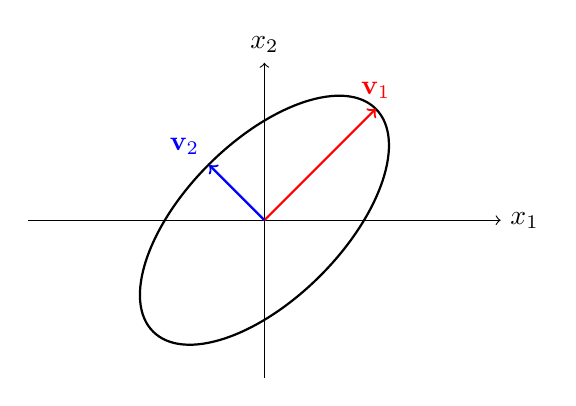
\begin{tikzpicture}
            % Draw the axes
            \draw[->][black] (-3,0) -- (3,0) node[right] {$x_1$};
            \draw[->][black] (0,-2) -- (0,2) node[above] {$x_2$};
            
            % Draw the ellipse
            \draw[black][rotate around={45:(0,0)}, thick] (0,0) ellipse (2 and 1);
            
            % Draw principal components
            \draw[->, red, thick] (0,0) -- (1.414, 1.414) node[above] {$\mathbf{v}_1$};
            \draw[->, blue, thick] (0,0) -- (-0.7, 0.7) node[above left] {$\mathbf{v}_2$};
            
        \end{tikzpicture}
        \caption{Principal Component Analysis (PCA) Ellipsoid. The red arrow indicates the first principal component (eigenvectors) $\mathbf{v}_1$ and the blue arrow indicates the second principal component $\mathbf{v}_2$.}
        \label{fig:pca_ellipsoid}
    \end{figure}
    
\end{remark}

%%%%%%%%%%%%%%%%%%%%%%%%%%%%%%%%%%%%%%%
\subsubsection{General transformations}

Suppose we transform the random vector $\X=(X_1,\dots,X_p)^\top$ into $\Y=g(\X)$. If the function $g$ is one-to-one and has differentiable inverse $u$, then 
\begin{equation*}
    f_{\Y}(\y) = |\det{\boldsymbol{J}}| f_{\X} (u(\y))
\end{equation*}
where 
$$
    \boldsymbol{J} = \brac{\frac{\partial u_i (y)}{\partial y_j}}_{i,j=1,\dots,p}
$$
is the \term{Jacobian matrix}. An important special case is that of linear transformations $\Y = \mA\X + \mb$. If $\mA$ is non-singular the inverse transform is $\X = \mA^{-1}(\Y-\mb)$ and $\boldsymbol{J} = \mA^{-1}$, so we obtain:
\begin{equation*}
    f_{\Y}(\y) = |\det{\mA^{-1}}| f_{\X} (\mA^{-1}(\y-\mb)).
\end{equation*}

%%%%%%%%%%%%%%%%%%%%%%%%%%%%%%%%%%%%%%%
%\subsection*{Lecture 4}
\subsection{Characteristic function}

In the univariate case we often studied the \term{moment generating function}:
$$
    M_X(t) = \ev{e^{tX}}.
$$
Important properties include:
\begin{enumerate}
    \item $M_X = M_Y \Rightarrow X \overset{d}{=} Y$,
    \item $\ev{X^k} = M^{(k)}_X(0)$,
    \item Independence of $X, Y$ implies $M_{X+Y} = M_X M_Y$.
\end{enumerate}
However, it does noe exist for for instance the student-t distribution. It only exists when all moments exist. We shall now define the \term{characteristic function}, which \textbf{always} exists:
$$
    \phi_X(t) = \ev{e^{itX}} = \int_\mathbb{R} f(x) e^{itx} dx.
$$
It has similar properties:
\begin{enumerate}
    \item $\phi_X = \phi_Y \Rightarrow X \overset{d}{=} Y$,
    \item $\ev{X^k} = i^{-k} \phi^{(k)}(0)$,
    \item Independence of $X, Y$ implies $\phi_{X+Y} = \phi_X \phi_Y$.
\end{enumerate}
In the p-variate case, the functions are functions of $\mt=(t_1,\dots,t_p)^\top$. Let as usual $\X=(X_1,\dots,X_p)^\top$ be our random vector. We define:
\begin{align*}
    M_{\X}(\mt) = \ev{e^{\mt^\top \X}}, \\
    \phi_{\X}(\mt) = \ev{e^{i\mt^\top \X}}.
\end{align*}
We list some important properties.
\begin{enumerate}
    \item If $\phi_{\X}(t)$ is absolutelly integrable, the (Fourier) inversion formula holds:
    $$
        f_{\X}(\x) = \frac{1}{(2\pi)^p} \int_{\R^p} e^{-i\mt^\top\x} \phi_{\X}(\mt) d\mt.
    $$
    \item Denote $t_{(1)} = (t_1,\dots,0)^\top, \dots, t_{(p)}=(0,\dots,t_p)^\top$. Then 
    $$
        \phi_{\X_k}(t_k) = \ev{e^{it_1 X_1}} = \ev{e^{i\mt_{(1)}^\top \X}} =  \phi_{\X}(t_{(k)}).
    $$
    \item Let $\X=\begin{pmatrix} \X_1 \\ \X_2 \end{pmatrix}$ and $\mt=\begin{pmatrix} \mt_1 \\ \mt_2 \end{pmatrix}$ be vectors with appropriate dimensions. Then:
    \begin{equation}
        \boxed{\X_1, \X_2 \textrm{ are independent } \Leftrightarrow \phi_{\X}(\mt) = \phi_{\X_1}(\mt_1)\phi_{\X_2}(\mt_2)}
    \end{equation} 
    \item Let $\X, \Y$ be independent p-variate random vectors. Then:
    $$
        \phi_{\X+\Y}(\mt) = \phi_{\X}(\mt)\phi_{\Y}(\mt).
    $$
\end{enumerate}
We end the section with a theorem linking the distributions of 1D random variables to the distribution of the p-variate random vector $\X$:
\begin{theorem}
    \term{Cramer-Wold} theorem states that the distribution of $\X\in\R^p$ is completelly determined by the set of all 1D distributions of $\mt^\top\X, \mt\in\R^p$.
\end{theorem}
\begin{proof}
    Suppose that for all $\mt\in\R^p$ we have $\mt^\top \X \overset{d}{=} \mt^\top \Y$. Then:
    $$
        \mt^\top \X \overset{d}{=} \mt^\top \Y \Rightarrow \phi_{\mt^\top\X}(u) = \phi_{\mt^\top\Y}(u).
    $$
    Taking $u=1$ gives $\ev{e^{i\mt^\top\X}} = \ev{e^{i\mt^\top\Y}}$ for all $\mt$, so $\phi_{\X}=\phi_{\Y}$ and hence $\X \overset{d}{=}  \Y$.
\end{proof}